%!TEX program = xelatex

\documentclass[compress]{beamer}
%--------------------------------------------------------------------------
% Common packages
%--------------------------------------------------------------------------
\usepackage[english]{babel}
\usepackage{pgfpages} % required for notes on second screen
\usepackage{graphicx}
\usepackage{subfigure}
\usepackage{multicol}
\usepackage{color}

%\usepackage[demo]{graphicx}
%\usepackage{caption}
%\usepackage{subcaption}

\usepackage{tabularx,ragged2e}
\usepackage{booktabs}

\usepackage{setspace}

%--------------------------------------------------------------------------
% Load theme
%--------------------------------------------------------------------------
\usetheme{hri}

\usepackage{dtklogos} % must be loaded after theme
\usepackage{tikz}
\usetikzlibrary{calc,mindmap,backgrounds,positioning,svg.path}



\graphicspath{{figs/}}

\renewcommand{\bf}{\Medium}

\newcommand\given[1][]{\:#1\vert\:}

%--------------------------------------------------------------------------
% General presentation settings
%--------------------------------------------------------------------------
\title{Mutual Modelling in Educational Child-Robot Interaction}
\subtitle{\textit{Does a second level of modelling\\enable higher quality interactions?}}
\date{EDRS candidacy exam}
\author{Alexis D. Jacq}
\institute{Computer-Human Interaction\\for Learning and Instruction {\Medium
EPFL}\\
\& Instituto Sup\'erior T\'ecnico\\  {\Medium
University of Lisbon}}

%--------------------------------------------------------------------------
% Notes settings
%--------------------------------------------------------------------------
%\setbeameroption{show notes on second screen}
%\setbeameroption{hide notes}

\begin{document}

\maketitle

%%%%%%%%%%%%%%%%%%%%%%%%%%%%%%%%%%%%%%%%%%%%%%%%%%%%%%%%%%%%%%%%%%%%%%%%%%%%%%%
%%%%%%%%%%%%%%%%%%%%%%%%%%%%%%%%%%%%%%%%%%%%%%%%%%%%%%%%%%%%%%%%%%%%%%%%%%%%%%%
%%%%%%%%%%%%%%%%%%%%%%%%%%%%%%%%%%%%%%%%%%%%%%%%%%%%%%%%%%%%%%%%%%%%%%%%%%%%%%%

\section{Introduction}
\begin{frame}{The CoWriter activity}
	\begin{figure}
        \centering
        \includegraphics[width=0.8\columnwidth]{experimental_setup}
    \end{figure}
\end{frame}

\begin{frame}{Henry interacting with Nao}
    \centering
    \includegraphics[width=0.5\columnwidth]{videos/test.png}
    \video{0.5\textwidth}{videos/test.mp4}
    \footnotemark{Jacq, A., Lemaignan, S., Garcia, F., Dillenbourg, P., Paiva, A.
    \textit{Building Successful Long Child-Robot Interactions in a Learning Context}
    HRI 2016}
\end{frame}

\begin{frame}{Limits}
\textbf{We don't know if the child understand exactly what we want him to understand.}
\begin{itemize}
\item The robot needs to be able to show that he did not understood eventual miss-behaviours
\item The learning speed of the robot may be too hight or too small
\item The robot could have micro-behaviour based on the content of the interaction
\item Sometimes we can lose the commitment of the child, that could be solve by a simple reaction of the robot
\end{itemize}
\end{frame}

\begin{frame}{Limits}
\begin{itemize}
\item The robot must be aware of the mind of the child
\item It must react to his image in the eyes of the child 
\item It needs an ``artificial theory of mind"
\end{itemize}
\end{frame}

\section{Mutual modelling in HRI}

\begin{frame}{Level 1}
    \begin{figure}
        \centering
        
\includegraphics[width=0.7\columnwidth]{naoMM}
        \caption{The robot building a model of the child: a first level of mutual modelling.}
    \end{figure}
\end{frame}

\begin{frame}{Level 2}
    \begin{figure}
        \centering
        \includegraphics[width=0.7\columnwidth]{naoMM2}
        \caption{The robot building a model of itself perceived by the child: a second level of mutual modelling.}
    \end{figure}
\end{frame}

%%%%%%%%%%%%%%%%%%%%%%%%%%%%%%%%%%%%%%%%%%%%%%%%%%%%%%%%%%%%%%%%%%%%%%%%%%%%%%%%%
\section{Framework}

\begin{frame}{Notations}
\begin{figure}[!tbp]
	\begin{minipage}[b]{.4\textwidth}
		
\includegraphics[width=0.8\columnwidth]{naoMM}
		\caption{\textcolor{blue}{$\textbf{M}_{\textbf{C}}$} (1st level)}
	\end{minipage}
	\hfill
	\begin{minipage}[b]{.4\textwidth}
		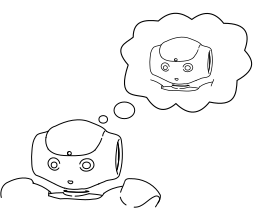
\includegraphics[width=0.8\columnwidth]{naoMM4}
		\caption{\textcolor{blue}{$\textbf{M}_{\textbf{R}}$} (1st level)}
	\end{minipage}
	\hfill
	\begin{minipage}[b]{.4\textwidth}
		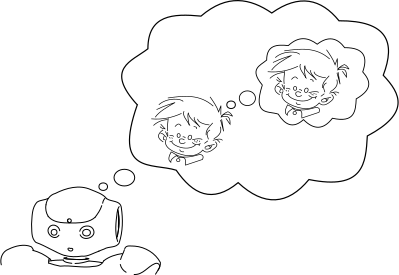
\includegraphics[width=0.8\columnwidth]{naoMM3}
		\caption{\textcolor{blue}{$\textbf{M}_{\textbf{C,C}}$} (2nd level)}
	\end{minipage}
	\hfill
	\begin{minipage}[b]{.4\textwidth}
		\includegraphics[width=0.8\columnwidth]{naoMM2}
		\caption{\textcolor{blue}{$\textbf{M}_{\textbf{C,R}}$} (2nd level)}
	\end{minipage}
	
\end{figure}

% faire les 4 !!

\end{frame}


\begin{frame}{Expected causalities}
$$ \mathbb{P}\left[\textit{mental state}\,\given[\Big]\,\textit{behaviour}\right]$$
$$ \mathbb{P}\left[\textit{abstract variables}\,\given[\Big]\,\textit{perveived variables}\right]$$
\end{frame}

\begin{frame}{Expected causalities}
$$M_{C}:$$
$$ \mathbb{P}\left[ \textit{Understand pointing} \given[\Big] \textit{look at the hand but not at the target}\right]\sim 0$$\\
$$ M_{C,R}:$$
$$ \mathbb{P}\left[\textit{Understand robot's progress}\,\given[\Big]\,\textit{Positive feedback}\right]\sim 1$$
\end{frame}


%%%%%%%%%%%%%%%%%%%%%%%%%%%%%%%%%%%%%%%%%%%%%%%%%%%%%%%%%%%%%%%%%%%%%%%%%%%%%%%%
\section{Cognitive architecture}

\begin{frame}{Global description}
	\begin{figure}
        \centering
        \includegraphics[width=1\columnwidth]{archi_already}
    \end{figure}
\end{frame}

\begin{frame}{Decision making}
\begin{enumerate}
\item \textcolor{blue}{Wizard-of-Oz}: A human takes decisions; the robot learns
\item \textcolor{blue}{Mixed-initiative}: The robot makes suggestions; a human agrees or disagrees
\item \textcolor{blue}{Autonomous}: The robot makes decisions
\end{enumerate}
\end{frame}

\begin{frame}{what is already here ?}
	\begin{figure}
        \centering
        \includegraphics[width=0.8\columnwidth]{screenshot.jpg}
        \caption{online \textit{with-me-ness}}
        \footnotemark{Lemaignan, S. and Garcia, F. and Jacq, A. and Dillenbourg, P.
    \textit{From Real-time Attention Assessment to “With-me-ness” in Human-Robot Interaction}
    HRI 2016}
    \end{figure}
\end{frame}

\begin{frame}{what is already here ?}
    \begin{figure}
        \centering
        % buttons
        \includegraphics[width=0.9\columnwidth]{buttons.jpg}
        \caption{Buttons for feedback}
    \end{figure}
\end{frame}

%%%%%%%%%%%%%%%%%%%%%%%%%%%%%%%%%%%%%%%%%%%%%%%%%%%%%%%%%%%%%%%%%%%%%%%%%%%%%%%%
\section{Implementation}

\begin{frame}{ROS nodes}
	\begin{figure}
        \centering
        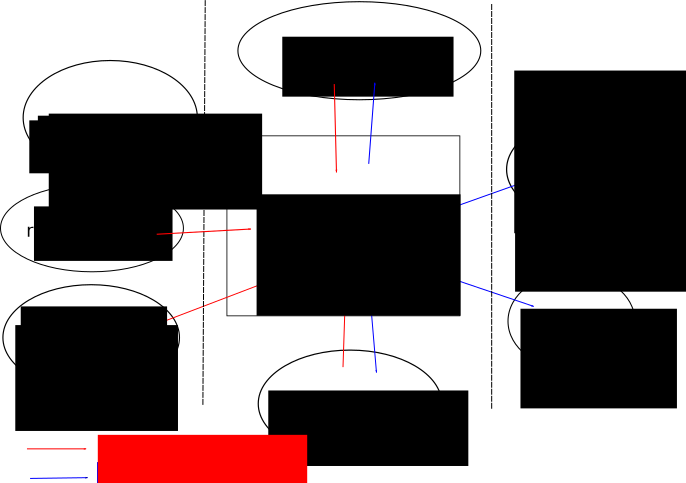
\includegraphics[width=0.8\columnwidth]{ros}
    \end{figure}
\end{frame}

%%%%%%%%%%%%%%%%%%%%%%%%%%%%%%%%%%%%%%%%%%%%%%%%%%%%%%%%%%%%%%%%%%%%%%%%%%%%%%%%
\section{Evaluation}

\begin{frame}{hypothesis}
\begin{itemize}
	\item \textit{Decisions made using additive information from second level of mutual modelling improve the quality of the CoWriter interaction.}
\end{itemize}
\end{frame}

\begin{frame}{Quality of the interaction ?}
\begin{enumerate}
	\item Quantity of demos
	\item Time spent to write demos
	\item Progress of child/robot
	\item With-me-ness
	\item Feedback buttons 
\end{enumerate}
\end{frame}

\begin{frame}{Experimental studies}
\begin{itemize}
	\item Long-term studies
	\item Children with real deficits
	\item Professional facilitators
\end{itemize}
\end{frame}

%%%%%%%%%%%%%%%%%%%%%%%%%%%%%%%%%%%%%%%%%%%%%%%%%%%%%%%%%%%%%%%%%%%%%%%%%%%%%%%%
\section{Conclusion \& planning}

\begin{frame}{Remind}
\begin{enumerate}
\item \textcolor{blue}{Question}: Does a second level of modelling\\enable higher quality interactions?
\item \textcolor{blue}{Hypothesis}: Yes.
\item \textcolor{blue}{Tools}: CoWriter activity + MM-cognitive architecture
\item \textcolor{blue}{Evaluation}: Long-term studies with children
\end{enumerate}
\end{frame}

\begin{frame}{Step by step approach}
\textbf{New variable (or group of variables) $\rightarrow$ New experiment to test the impact}
	\begin{figure}
        \centering
        \includegraphics[width=1\columnwidth]{archi_newstep}
    \end{figure}
\end{frame}

\begin{frame}
	\begin{figure}
        \centering
        \includegraphics[width=1.\columnwidth]{robots}
    \end{figure}
\end{frame}

\end{document}






